\RequirePackage{plautopatch}
\documentclass[12pt,a4paper,report,uplatex,dvipdfmx]{jsbook}
\usepackage{mediathesis} % 卒論用パッケージ

%% Include path の設定
\graphicspath{{fig/}} %% グラフィック用
%\makeatletter
%\providecommand*{\input@path}{}
%\g@addto@macro\input@path{{src/}}% tex ソースファイル用
%\makeatother

%%%%%%%%%%%%%%%%%%%%%%%%%%%%%%%%%%%%%%%%%%%%%%%%%%%%%%%%%%%%%%%%%%%%%%%%%%%%%%%%%%%%
%%%% タイトル・概要設定 %%%%
% 提出年度(西暦)
\YearH{2022}



% 提出年(西暦)
\BringYear{2023}

% 提出月
\BringMonth{1}

% タイトル
\PaperTitle{リアルタイム 3DCG における}

% タイトル二行目(省略可)
\PaperTitleII{\LaTeX サンプルに関する研究}

% 著者名
\AuthorName{三次元 萌子}

% 学籍番号
\AuthorNumber{M01xxxxx}

% 指導教員名
\TeacherName{渡辺 大地 教授}

% 卒研プロジェクト名
\ProjectName{ゲームサイエンスプロジェクト}

% キーワード
\KeyWordsI{三次元、温度差、無礼講、}

% キーワード二行目(省略可、二行目を利用する場合は一行目の最後を読点で終わること)
\KeyWordsII{年齢差、軋轢}

% タイトル図ファイル
\TitleFig{titlems.eps}



% 概要
\Abstract{
近年、リアルタイム 3DCG アプリケーションの構築が盛んに行なわれているが、
その際に学部生と院生の間で生じる温度差が問題となっている。
これは、教員と学生との軋轢を生じる原因となり、深刻な状況に発展する場合もある。
本研究では、まずこのような問題の原因を探り、原因の特定を行なった。
さらに、「年齢差吸収理論」や「無礼講技能」の手法を応用することで、温度差を急激に収束することを示した。
この手法を二つの研究プロジェクトにおいて実験し、手法が有効であることを示した。

アブストラクト中でも改段落については本文と同様に扱う。
つまり、強制改行と全角スペースによる強制補正は禁止である。

}


%%%%%%%%%%%%%%%%%%%%%%%%%%%%%%%%%%%%%%%%%%%%%%%%%%%%%%%%%%%%%%%%%%%%%%%%%%%%%%%%%%%%
%%%% 寸法設定 %%%%

\setlength{\textwidth}{170truemm}		% 本文横幅
\setlength{\textheight}{230truemm}		% 本文縦幅
\setlength{\topmargin}{-5truemm}		% 上部マージン調整
\setlength{\oddsidemargin}{-4truemm}		% 奇数ページ左余白
\setlength{\evensidemargin}{\oddsidemargin}	% 偶数ページ左余白
\setlength\abovecaptionskip{-0.5truemm}		% 図キャプションと図との間隔
\setlength\belowcaptionskip{1.5truemm}		% 表キャプションと表との間隔

%%%% 各種マクロ例 %%%%

\newcommand{\bez}{\mbox{$\mathrm{B \acute{e} zier}$}}
\newcommand{\dw}[2]{\mbox{$\mathrm{{#1}_{#2}}$}}
\newcommand{\uw}[2]{\mbox{$\mathrm{{#1}^{#2}}$}}

%%%% PDF ハイパーリンク各種設定 %%%%

\hypersetup{
        bookmarksnumbered=true,
        colorlinks=false,
        setpagesize=false
}


%%%%%%%%%%%%%%%%%%%%%%%%%%%%%%%%%%%%%%%%%%%%%%%%%%%%%%%%%%%%%%%%%%%%%%%%%%%%%%%%%%%%
% ここより本文開始

\begin{document}

\pagewiselinenumbers		% 行番号付加 (本番印刷の際はコメントアウト)

\MediaThesisTitle		% タイトル作成

\pagenumbering{Roman}		% 目次用ページスタイル
\tableofcontents		% 目次
\listoffigures			% 図目次(必要に応じて有効化/無効化)
%\listoftables			% 表目次(必要に応じて有効化/無効化)
\clearpage
\pagenumbering{arabic}		% 本文用ページスタイル
\pagestyle{plain}		% 本文ページ番号位置
\baselineskip=23pt		% 行間設定

% ここから本文ファイルを挿入

\chapter{はじめに}
\label{chp:first}

\section{段落と改行}
\label{sec:paragraph}

段落頭の字下げは自動で行われるため、全角スペースによる手動調整は不要であり、禁止である。
\LaTeX ソース中での改行は空行を挟まない場合は無視される。
ソース内では自分で編集しやすいように改行してよい。

このように、空行を挟むと改段落となる。
また、強制改行は\\このように \verb+\\+ で強制的に行うことができる。
しかし、この場合は段落の字下げもされないため、改段落を行う用途には空行を用いるべきで、
強制改行(\verb+\\+)は利用すべきではない。

しかしながら、例えば \verb+\verb+ 環境やインライン数式を用いる場合などで、
\verb+abcdefghijklmnopqrstuvwxyzABCDEFGHIJKLMNOPQRSTUVWXYZ+ 
というようにページ幅を超えてしまったり、前の行が間延びしてしまうようなケースがある。
そのような場合、\verb+\\+ を用いて強制改行により \\
\verb+abcdefghijklmnopqrstuvwxyzABCDEFGHIJKLMNOPQRSTUVWXYZ+ 
というように用いるとよい。

\section{箇条書き}
\label{sec:enum}

数字を使った場合の箇条書きの例を示す。

\begin{enumerate}
 \item 数字の付いた箇条書きの例
 \item こんな感じで手順などを列挙
\end{enumerate}

数字を付けずに列挙したい場合は itemize 環境を使う。
このようにあるキーワードを指定して \verb+\begin(}+ と \verb+\end{}+ で
囲む範囲のことを○○環境と呼ぶ。

\begin{itemize}
 \item 順番などを伴わない箇条書きの例
 \item 材料や要素を純粋に列挙したい場合に使用
\end{itemize}

enumerate 環境や itemize 環境は、入れ子構造を持つことができる。
例えば enumerate 環境の場合、以下のようになる。
\begin{enumerate}
 \item 東京都
 \begin{enumerate}
  \item 八王子市
  \item 多摩市
 \end{enumerate}
 \item 神奈川県
 \begin{enumerate}
  \item 横浜市
  \item 川崎市
 \end{enumerate}
 \item 山梨県
\end{enumerate}

\section{図表と参照}
\label{sec:fig_tbl}

図を挿入する際は以下のように書く。
必ずキャプションを付けるとともに、図に対する説明を本文中で記載すること。
何かの手違いで図が表示されなくなったとしても、文章で意味が通じるくらいに説明するのを目安にすること。
以下の図 \ref{fig:sample} と図 \ref{fig:ferret} は、適当なサンプル画像である。

\begin{figure}[H]
  \centering
  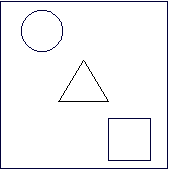
\includegraphics[width=6.4cm]{./fig/fig-sample.pdf}
  \caption{適当なサンプル}
% \url{http://www.this.is.sample.url/} % Web上のデータの場合、参照先URLを明記
  \label{fig:sample}
\end{figure}

\begin{figure}[H]
  \centering
  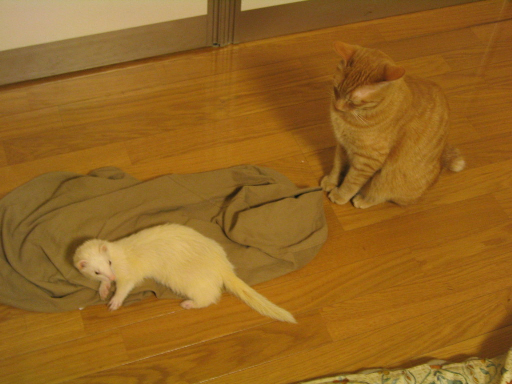
\includegraphics[width=6.4truecm]{./fig/ferret.png}
  \caption{適当なサンプル2}
% \url{http://www.this.is.sample.url/} % Web上のデータの場合、参照先URLを明記
  \label{fig:ferret}
\end{figure}

これまで、\LaTeX での図は伝統的には EPS 形式が用いられてきたが、
近年では JPEG 形式や PNG 形式など多くの画像フォーマットに対応している。
Inkscape や Illustrator 等のように直接 EPS 形式を出力する場合は EPS を用いることが望ましいが、
それ以外の状況では EPS への変換は行わずに画像ファイルを直接指定した方が品質が良い。
ただし、JPEG や PNG などの画像ファイルは EPS に比べて \LaTeX のコンパイルが長時間になる傾向があり、
あまり巨大な画像データを使用するとかなりコンパイル時間が長くなってしまうので、注意が必要である。
また、使用する画像ファイルはこのテンプレートのように
fig サブフォルダ内に格納することを推奨する。

図への参照は \verb+\label+ コマンドを用いて各図のキャプションにキーワードを付けておき、
文中で \verb+\ref+ コマンドによってキーワードを指定することで記述する。
キーワードは参照対象に応じてプリフィクスを付けることが望ましい。
以下の表 \ref{tbl:pre_list} に一般的に用いる参照対象ごとのプリフィクスを挙げる。

\begin{table}[H]
  \caption{ラベルに指定するキーワードのプリフィクス一覧}
  \label{tbl:pre_list}
  \centering
  \begin{tabular}{|l|l|r|} \hline
   参照対象	& プリフィクス \\ \hline
   章		& chp: \\ \hline
   節		& sec: \\ \hline
   図		& fig: \\ \hline
   表 		& tbl: \\ \hline
   式   	& eqn: \\ \hline
  \end{tabular}
\end{table}
手作業でのナンバリングは非効率極まりない上に必ずミスが出るので行わないこと。

\section{\LaTeX のコンパイル}
\LaTeX のコンパイルは、「コマンドプロンプト」や「PowerShell」などのコマンドライン上で「
latexmk」コマンドを用いる。
例えば、「M01xxyyy.tex」というファイルから PDF を作成したい場合は
\begin{verbatim}
    latexmk M01xxyyy
\end{verbatim}
というように、拡張子を抜いてコマンドラインで指定する。

また、コマンドラインに不慣れな学生は、
Atom エディタ等の \LaTeX パッケージを用いることも良案である。
Atom エディタを用いた \LaTeX の記述については、研究室 Wiki を参照のこと。
		% 第1章
\chapter{その次}
\label{chp:second}

\section{数式}
\label{sec:eqn}

数式のインラインモードは \(x^2 + y^2 \leq 1\) のように表示させることができる.
インラインモードで「\verb+$...$+」を使うやり方は,
近年の LaTeX ではあまり推奨されていないが,その利用は妨げない.

ディスプレイ数式モードを利用する際に推奨するのは equation 環境である.
\begin{equation}
	\mathbf{A}_p = \frac{\mathbf{A}\cdot\mathbf{B}}{|\mathbf{B}|^2}\mathbf{B} .
	\label{eq:samp1}
\end{equation}
数式の参照は「\verb+\ref+」ではなく「\verb+\eqref+」を用いる.
上記の数式を参照すると「式\eqref{eq:samp1}」となる.
このように,\verb+\eqref+ を用いた場合は数式中と同じ様式の括弧がつく.

また,複数行にわたる数式を表示したい場合は align 環境を用いることを推奨する.
以下の式\eqref{eq:samp2}にその例を示す.

\begin{align}
	& \begin{bmatrix}
	a_{11} & a_{12} & \cdots & a_{1n} \\
	a_{21} & a_{22} & \cdots & a_{2n} \\
	\vdots & \vdots & \ddots & \vdots \\
	a_{m1} & a_{m2} & \cdots & a_{mn} \\
	\end{bmatrix}
	\otimes
	\begin{bmatrix}
	b_{11} & b_{12} & \cdots & b_{1n} \\
	b_{21} & b_{22} & \cdots & b_{2n} \\
	\vdots & \vdots & \ddots & \vdots \\
	b_{m1} & b_{m2} & \cdots & b_{mn} \\
	\end{bmatrix} \notag \\
	& \qquad \qquad = \sum_{i}^{m}\sum_{j}^{n}a_{ij}b_{ij} .
	\label{eq:samp2}
\end{align}

数式で複数行を用いる方法として、古い \LaTeX に関する資料では eqnarray 環境の
解説を行っている場合があるが、最近の \LaTeX では幾つかのパッケージ
(特に\AmS 関連)と同時に利用すると問題が発生することがあるため、利用は推奨しない.
複数行を用いる方法としては他にも gather, multline, split など多くの環境があるが、
equnarray 以外のものであれば問題はない。

具体的な数式の記述方法については書籍や Web 上の情報等を参照のこと。

\section{寸法}

\LaTeX では、縦方向や横方向に空白を空けたいとき (\verb+\vspace+, \verb+\hspace+) や、
画像の縦幅や横幅を指定したい場合など、多くの場面で寸法を指定することがある。
\LaTeX の寸法単位は mm (ミリメートル) や cm (センチメートル) など多くの種類が利用でき、
小数点以下も記述できるためかなり柔軟な指定ができる。例えば、表のキャプションと
本体の間を少し空けたいときは
\begin{verbatim}
\begin{table}[H]
  \caption{ラベルに指定するキーワードのプリフィクス一覧}
  \label{tbl:pre_list}
  \centering
  \vspace{0.5cm}
  \begin{tabular}{|l|l|r|} \hline
\end{verbatim}
のように、表本体の直前に \verb+\vspace+ を入れればよい。

\LaTeX の寸法指定で留意すべきこととして、単位の「true つき」と「true なし」の使い分けがある。
例えば、先述の「\verb+\vspace{0.5cm}+」に対し、true つきの場合は
「\verb+\vspace{0.5truecm}+」ということになる。

true がついていない場合、\verb+\documentclass+ の指定時でのフォントサイズを変更すると、
そのフォントサイズに伴って(空白幅や画像幅などの)実際の寸法も変化する。
フォントサイズを変更した際に連動してほしい寸法については、この「true なし」を用いるとよい。
一方、「true つき」の場合はフォントサイズの変更には連動せず常に固定の値となる。
センタリングした画像幅などはフォントサイズと連動しない方が都合がよいことも多く、
そういった場合は「true つき」の寸法を指定するとよい。

\section{参考文献}
\label{sec:bib}

参考文献リストの作成は、\BibTeX を用いることを推奨する。
文献の参照は、リスト上で文献に付けたキーワードをciteコマンドによって指定することで記述する。
例えば、
「阿部ら\cite{abeJ}によると、
某手法\cite{nowrouzezahrai}には重大な欠点が存在することが指摘されている。」
という利用方法となる。

文献を1つも参照していない状態でPDFを生成するバッチファイルを実行するとエラーとなるので注意すること。
生成したPDFファイル中で参照がうまくできていない場合には参照番号ではなく
「\verb+?+」記号が表示される。

\BibTeX の記述方法は、どのような種類の文献かによって異なる。以下に具体的な例を列挙する。
\begin{itemize}
 \item 論文誌掲載の学術論文\cite{abeJ}\cite{nowrouzezahrai}
 \item 研究会の研究報告\cite{aoki}
 \item 博士論文\cite{takeuchi}
 \item 修士論文\cite{abeM}
 \item 学部卒業論文\cite{abeU}
 \item 書籍\cite{dragonball}
 \item URL\cite{effekseer}
\end{itemize}

文献の属性の種類や、設定するべきステータスについてもWebを参照すること。
論文データベースサイトでは \BibTeX の記述形式によるテキストを出力してくれるところもあるので、
利用できると便利である。
リストの記述順は一切気にする必要がなく、
参考文献に挙げないものが含まれていても問題無いので、関連しそうな文献は全てリスト化しておくとよい。

\BibTeX における著者名の列挙はカンマで並べるのではなく、
\begin{verbatim}
    author = "阿部 雅樹 and 渡辺 大地 and 三上 浩司",
\end{verbatim}
というように、各氏名の間に「and」を入れるという独特の形式を持つ。

また、\BibTeX では author や title 等での
アルファベット大文字小文字を自動的に変換する機能があり、
例えばタイトル中の「3DCG における」といった文字列は「3dcg における」となる。
これを強制的に大文字小文字を指定したい場合は、
\begin{verbatim}
    title = "{3DCG}における何かしらの手法",
\end{verbatim}
のようにその部分だけ波括弧で囲うことで指定できる。

			% 第2章

\delchapnumber
\chapter{謝辞}
\label{chp:thanks}

謝辞は基本的に査読の対象とならない。各人の自由に記述して良い。
ただし、あまりに公序良俗に反する内容である場合は修正を求める場合があるので、
はっちゃけるにしても良識・常識の範疇を超えないようにして欲しい。
			% 謝辞
\bibliography{BibTeX}		% BibTeXを使う場合の参考文献リスト
\bibliographystyle{junsrt}	% BibTeXを使う場合のスタイル
\undochapnumber
% \appendix			% 付録 (もしあれば)
% \input{appendix}		% 付録ファイルの挿入

\end{document}
